In this section we break down the implementation of the system into its core components, following the methodology and requirements outlined in the previous sections. The full implementation can be found in the appendix \ref{chapter:appendix}.

The resulting system consists of two main components. The \textbf{APR core} which holds the core logic for the repair process. The second component is the 	\textbf{Continuous Integration Pipeline} which integrates the core logic within a GitHub repository. It serves as the entry point and orchestrates the execution of the APR core based on configured triggers events of the repository.

\section{System Components}
The implementation of the main components will be described in detail in the following section.

\textbf{APR Core:}

% agent architectures produce good results epically paired with containerized environments. \cite{puvvadiCodingAgentsComprehensive2025}
The APR core contains the main bug fixing logic written in Python\footnote{}. Embedding it into a Docker Image \footnote{} makes it easy to deploy, portable and small in memory. In order to use the APR core the following data (displayed in table \ref{tab:container-inputs}) needs to passed to the container:

\renewcommand{\arraystretch}{1.5} % Set row spacing to 1.5
\begin{longtable}{@{\extracolsep{\fill}} p{3.7cm} | p{7cm} | p{4cm}  @{}}
    \caption{Container Inputs} \label{tab:container-inputs}                                     \\

    \toprule
    \textbf{Name}      & \textbf{Description}                            & \textbf{Type}        \\
    \midrule
    \endfirsthead

    \bottomrule
    \endfoot
    Source Code        & Git repository where APR fix bugs               & Docker volume mount
    \\ \hline
    GITHUB\_TOKEN      & Token for GitHub API authentication             & Environment variable \\
    \hline
    LLM\_API\_KEY      & API key for the \ac{LLM} provider               & Environment variable \\
    \hline
    ISSUE\_TO\_PROCESS & The issue to process in JSON format             & Environment variable \\
    \hline
    GITHUB\_REPO       & GitHub repository for fetching and writing data & Environment variable \\
    \hline
\end{longtable}

With this environment set, the APR core iterates over all issues fetched from the ``ISSUE\_TO\_PROCESS'' environment variable. For each issue, the main APR logic is executed. This logic follows a predefined flow that makes use of multiple stages and tools.

First, a clean workspace and the issue repair context is set up. The context acts as the main data structure for the issue repair process and is used at every step. \ref{lst:context-json} shows what the context looks like when initialized.

\begin{lstlisting}[style=json, caption={Context JSON}, label={lst:context-json}]  
context = {
    "bug": issue,
    "config": config,
    "state": {
        "current_stage": None,
        "current_attempt": 0,
        "branch": None,
        "repair_successful": False,
    },
    "files": {
        "source_files": [],
        "fixed_files": [],
        "diff_file": None,
        "log_dir": str(log_dir),
    },
    "stages": {},
    "attempts": [],
    "metrics": {
        "github_run_id": os.getenv("GITHUB_RUN_ID"),
        "script_execution_time": 0.0,
        "execution_repair_stages" : {},
        "tokens": {}
    },
}
\end{lstlisting}

The context is passed between stages, with each stage performing a specific task in the bug fixing process and returning an updated context. The core stages are Localize, Fix, Build, and Test.

The repair process starts with the localization stage. This stage attempts to identify the files in the codebase required to fix the bug, using the configured \ac{LLM} via the provider's Software Development Kit (SDK). The localization prompt is built using the issue and a constructed hierarchy of the repository's file structure. The response is expected to return a list of files where the bug might be located. The localization system instruction and prompt are shown in \ref{lst:localization-prompt}.

\begin{lstlisting}[style=python, caption={Localization Prompt}, label={lst:localization-prompt}]
system_instruction = "You are a bug localization system. Look at the issue description and return ONLY the exact file paths that need to be modified."

prompt = f"""
    Given the following GitHub issue and repository structure, identify the file(s) that need to be modified to fix the issue.

    Issue #{issue['number']}: {issue['title']}
    Description: {issue.get('body', 'No description provided')}

    Repository files:
    {json.dumps(repo_files, indent=2)}

    Return a JSON array containing ONLY the paths of files that need to be modified to fix this issue.
    Example: ["path/to/file1.py", "path/to/file2.py"]
    """
\end{lstlisting}

With the localized files in context, the Fix stage comes next. This stage again uses the configured \ac{LLM} API to generate a fix for the issue in the localized files. The prompt includes the issue details and file names along with their content. The response is expected to contain a list of edits for each file. The \ac{LLM} may also specify that no changes are required in certain files. The generated response is then parsed and applied to the files in the workspace. Finally, the context is updated with the new file content. Below is the system instruction and base prompt used for the Fix stage \ref{lst:repair-prompt}.

\begin{lstlisting}[style=python, caption={Repair Prompt}, label={lst:repair-prompt}]
system_instruction = "You are part of an automated bug-fixing system. Please return the complete, corrected raw source files for each file that needs changes, never use any markdown formatting. Follow the exact format requested."

base_prompt = f"""
    The following Python code files have a bug. Please fix the bug across all files as needed.

    {files_text}

    Please provide the complete, corrected source files. If a file doesn't need changes, you can indicate that.
    For each file that needs changes, provide the complete corrected file content.
    Format your response as:

    === File: [filepath] ===
    [complete file content or "NO CHANGES NEEDED"]

    === File: [filepath] ===
    [complete file content or "NO CHANGES NEEDED"]
    """
    
\end{lstlisting}

For validating the generated edits, two stages are available: Build and Test. The Build stage is responsible for validating the syntax of the changes made in the Fix stage. It checks if the code can be built. For Python code, this means checking if all syntax is valid and follows standardized code quality and maintenance rules \footnote{todo}. To achieve this, the code is first formatted using the Python formatter Black\footnote{todo} and then linted using flake8\footnote{todo}. This ensures properly formatted code and appends any warnings or errors to the context.

After validation, the generated code is tested, if a test command is configured. The test stage runs the tests defined in the repository using the configured test command for each fixed file. In case tests fail, the context is updated with the error messages, and the repair returns to the Fix stage for a new attempt.

For a new attempt, additional feedback is generated using the previous code and stage results and attached to the prompt. When the maximum number of attempts is reached and the code still does not pass testing, an unsuccessful repair is reported to the issue by creating a comment using the GitHub API.

If validation and testing are successful, the issue is marked as successfully repaired. The file changes are committed and pushed to the remote repository. A Pull Request is then created to merge the issue branch into the main branch. This Pull Request includes detailed file diffs and links the issue.

At this point, integration with the GitHub repository is completed. During execution, the APR Core logs every action, which can be used for debugging and makes the repair process more transparent. Furthermore, it collects metrics such as the number of attempts, execution times, and token usage, which are essential for analyzing the effectiveness and performance of the APR system. A summary of the metrics is mentioned in \ref{section:evaluation}.

The APR core is designed to be modular and extensible, allowing for future enhancements and additional stages or tools to be integrated as needed. It is also designed to be lightweight, ensuring that it can run efficiently within a CI environment. Figure \ref{fig:apr-core} illustrates the functionalities (blue) and tools (green) used in the APR Core.

\begin{figure}[H]
    \centering
    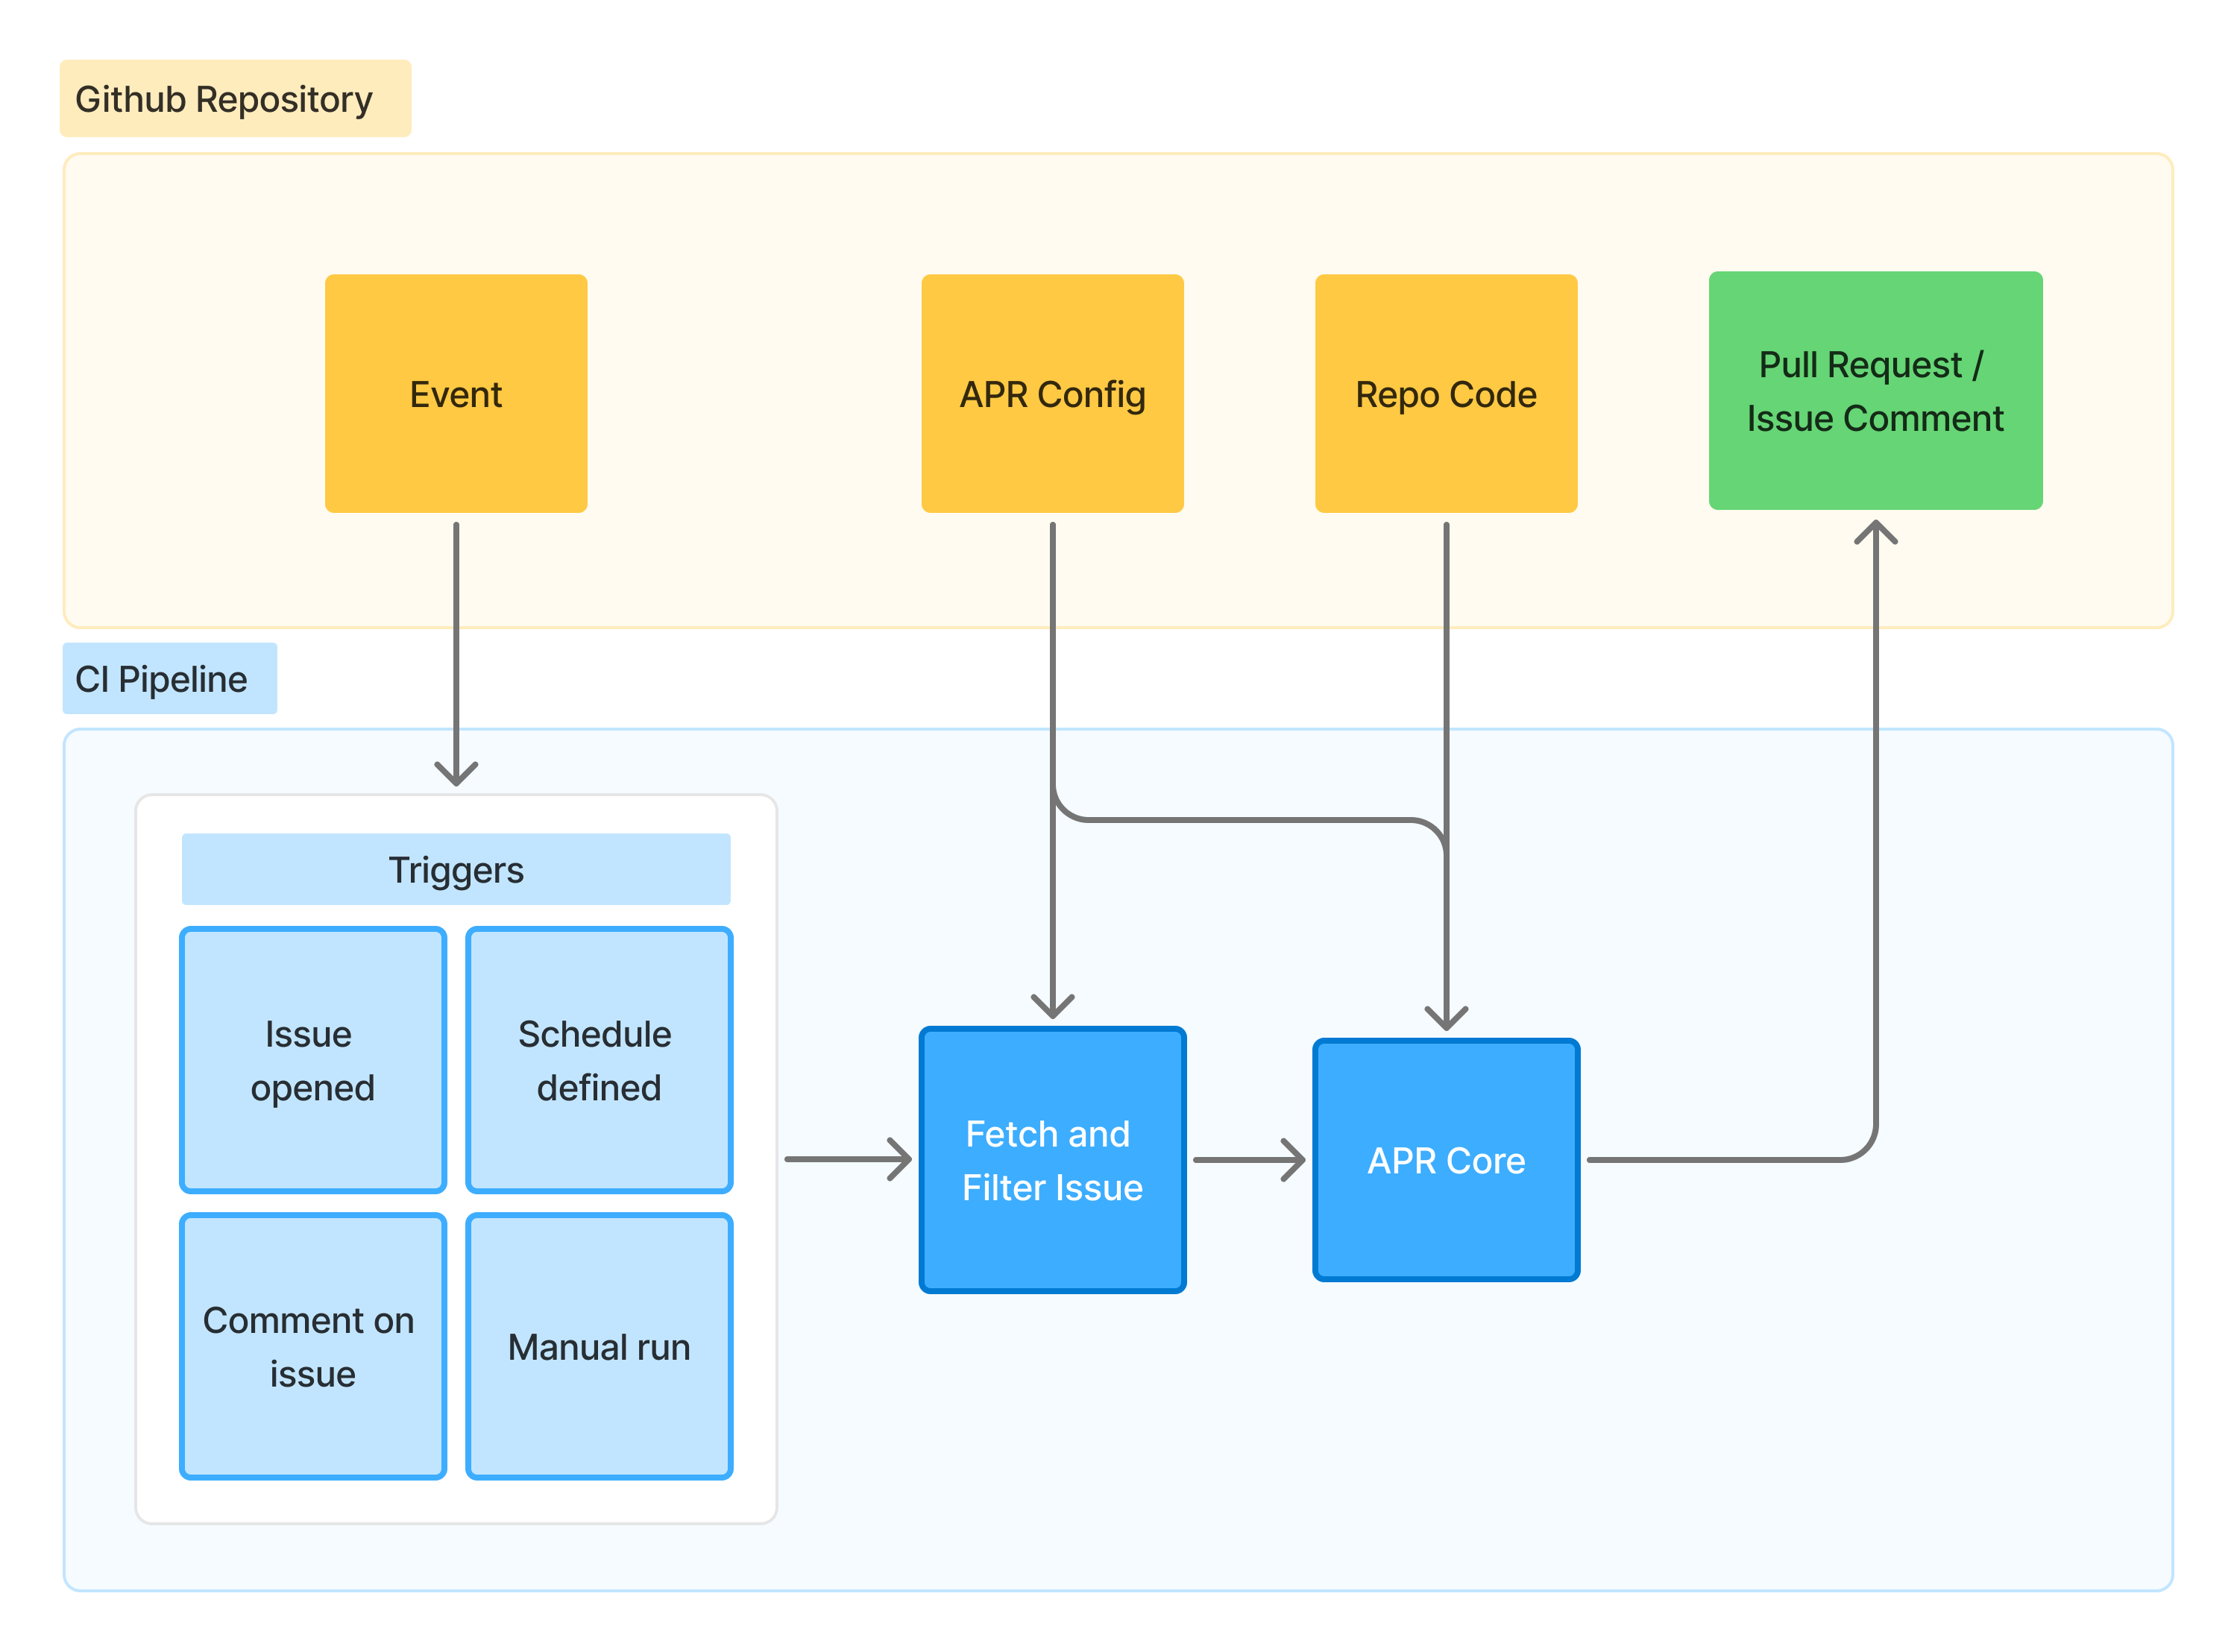
\includegraphics[width=1\textwidth]{images/flowcharts/apr_core.png}
    \caption{APR Core Logic}
    \label{fig:apr-core}
\end{figure}

\textbf{Continuous Integration Pipeline:}

A GitHub Action Workflow integrates the APR Core into the GitHub repository. The workflow is written in YAML\footnote{YAML is a human readable data serialization language. \cite{OfficialYAMLWeb}} according to the GitHub Action standard \cite{WorkflowSyntaxGitHub}. For this prototype, we use Linux x64 runners provided and hosted by GitHub. This eliminates the overhead of managing our own runners but comes at the cost of uncertain performance and availability.

The workflow is made up of multiple triggers and jobs. Triggers are based on events\footnote{explain and link} from the GitHub repository and serve as the entry point for executing the jobs. Given the triggers, the workflow can be executed in two different ways:

\begin{itemize}
    \item Batch processing by fetching all issues marked for repair. This can be triggered by a manual dispatch (``workflow\_dispatch'') or scheduled execution (``cron'').
    \item Processing a single issue from the event. The issue is passed from the (``issue\_labeled'') event when labeled with the configured labels or from (`'`issue\_comment'') when extra information is added to the issue in the form of a comment.
\end{itemize}

The trigger event information gets passed as environment variables to the first job named ``gate''. This job uses the data to determine if the issue should be processed or skipped using a Python script (``filter\_issues.py''). This script must be placed where it is accessible to the workflow file. It checks the labels of the issue and evaluates its state to determine if it is relevant for the APR process.

If no issues pass the ``gate'', the ``skipped'' job is executed, which simply logs that no issues were found and exits the workflow run. If issues do pass the ``gate'', the ``bugfix'' job is started. This job is responsible for executing the APR Core logic. It sets up the necessary prerequisites (see \ref{tab:container-inputs}) to start a container using the latest APR Core Docker Image, which performs the repair. These include checking out and mounting the code repository, setting environment variables, and providing the necessary permissions for the APR Core to edit repository content, create pull requests, and write to issues on GitHub.


The final step of `bugfix` is uploading the logs and metric files from the APR Core as artifacts, making them available after the workflow run has completed.

Figure \ref{fig:ci} visualizes the workflow and its jobs.

\begin{figure}[H]
    \centering
    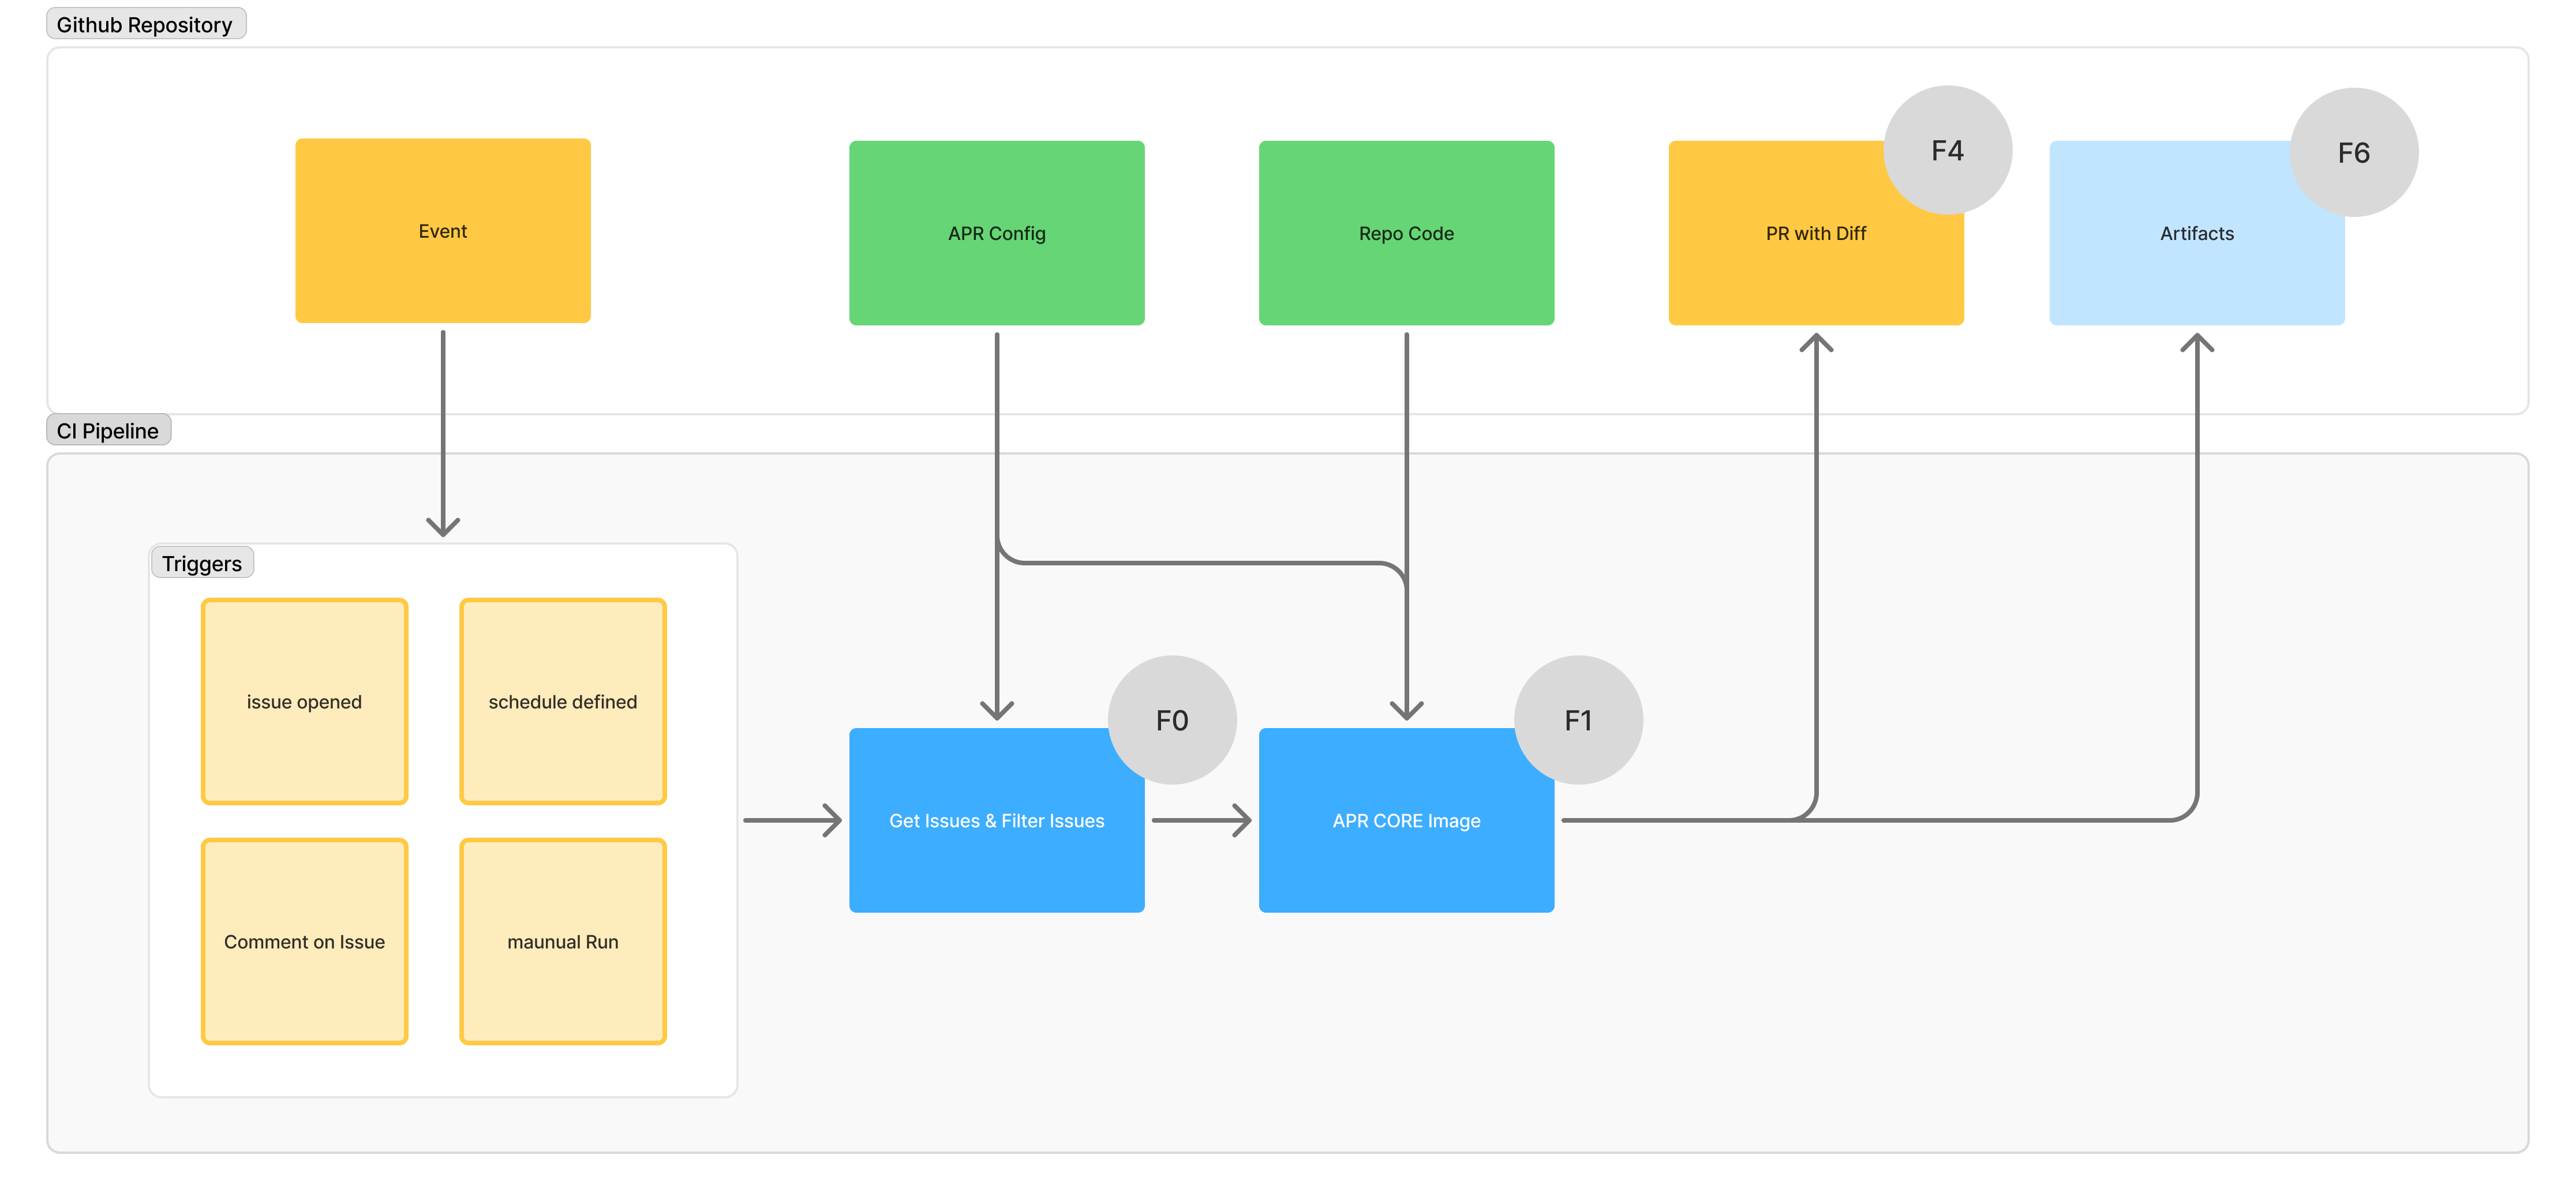
\includegraphics[width=1\textwidth]{images/flowcharts/ci.png}
    \caption{APR Core Logic}
    \label{fig:ci}
\end{figure}

To use this integration in a repository, the workflow file must be placed in the ``.github/workflows'' directory of the repository along with ``filter\_issues.py'' in ``.github/scripts''. With this in place, an ``LLM\_API\_KEY'' must be set as a secret in the repository settings. This key is used by the APR Core to authenticate with the configured \ac{LLM} provider API. Lastly, GitHub Actions must be granted permissions to create pull requests and write to issues in the repository. This is done by setting the workflow permissions in the repository settings under Actions -> General -> Workflow permissions.

\section{System Configuration}
%TODO add  collision avoidance
To make the system easily adjustable, the APR Core and the CI Pipeline can be configured using a YAML configuration file. This configuration is optional, when no configuration is provided, the system uses a default setup. A custom configuration must be named ``bugfix.yml'' and placed at the root of the repository. This setup allows for easy customization of the system without modifying the code. The configuration is read by system components during execution. Table \ref{table:configuration} lists the available configuration fields along with their descriptions.

\renewcommand{\arraystretch}{1.5}
\begin{longtable}{@{\extracolsep{\fill}} p{3.5cm} | p{11cm} @{}}
    \caption{Configuration Fields and Descriptions} \label{table:configuration}                        \\
    \toprule
    \textbf{Configuration Field} & \textbf{Description}                                                \\
    \midrule
    \endfirsthead

    \bottomrule
    \endfoot

    to\_fix\_label               & The label used to identify issues that need fixing.                 \\ \hline
    submitted\_fix\_label        & The label applied to issues when a fix is submitted.                \\ \hline
    failed\_fix\_label           & The label applied to issues when a fix fails.                       \\ \hline
    workdir                      & The working directory where the code lives.                         \\ \hline
    test\_cmd                    & The command used to run tests on the codebase.                      \\ \hline
    branch\_prefix               & The prefix for branches created for bug fixes.                      \\ \hline
    main\_branch                 & The main branch of the repository where bug fix branches are based. \\ \hline
    max\_issues                  & The maximum number of issues to process in a single run.            \\ \hline
    max\_attempts                & The maximum number of attempts to fix an issue.                     \\ \hline
    provider                     & The \ac{LLM} provider used for generating fixes.                    \\ \hline
    model                        & The specific model from the \ac{LLM} provider.                      \\
\end{longtable}



\section{Requirement Validation}

This section demonstrates how the prototype satisfies the functional and non-functional requirements defined in Chapter \ref{chapter:requirements}. Table \ref{tab:req-validation} summarizes the satisfaction and verification of the requirements with provided screenshots, context excerpts and log excerpts captured during development. Full logs, configuration files, and context JSON files for all runs referenced available in the GitHub repositories listed in the Appendix \ref{chapter:appendix}.


\renewcommand{\arraystretch}{1.5}
\begin{longtable}{@{\extracolsep{\fill}} p{0.5cm} | p{3.5cm} | p{1.5cm} | p{6cm} @{}}
    \caption{Requirement Satisfaction and Validation} \label{tab:req-validation}                                                                                                                                                                      \\
    \hline
    \textbf{ID} & \textbf{Title}                      & \textbf{Satisfied} & \textbf{Verification / Reference}                                                                                                                                        \\
    \hline
    \endfirsthead

    \hline
    \endfoot

    F0          & Multiple Triggers                   & Yes                & See Figure~\ref{fig:triggers}.                                                                                                                                           \\ \hline
    F1          & Issue Filtering                     & Yes                & See filtered issues log in Listing~\ref{lst:filtered-issues}.                                                                                                            \\ \hline
    F2          & Code Checkout                       & Yes                & See log excerpt in Listing~\ref{fig:code-checkout}.                                                                                                                      \\ \hline
    F3          & Bug Localization                    & Yes                & See log excerpt in Listing~\ref{lst:loc}.                                                                                                                                \\ \hline
    F4          & Fix Generation                      & Yes                & See context excerpt in Listing~\ref{fig:fix}.                                                                                                                            \\ \hline
    F5          & Change Validation                   & Yes                & See log excerpt in Listing~\ref{fig:validation}.                                                                                                                         \\ \hline
    F6          & Iterative Patch \newline Generation & Yes                & See log excerpt in Listing~\ref{fig:retry}.                                                                                                                              \\ \hline
    F7          & Patch Application                   & Yes                & See og excerpt in Listing~\ref{lst:branch-commit}.                                                                                                                       \\ \hline
    F8          & Result Reporting                    & Yes                & See Figure~\ref{fig:pr-report} and Figure \ref{fig:comment}.                                                                                                             \\ \hline
    F9          & Log and Metric \newline  Collection & Yes                & See Figure~\ref{fig:logs-artifacts}.                                                                                                                                     \\ \hline
    N1          & Container Runtime                   & Yes                & See log excerpt in Listing~\ref{lst:docker-log}.                                                                                                                         \\ \hline
    N2          & Configurable                        & Yes                & See log excerpts from Listing \ref{lst:load-config}.                                                                                                                     \\ \hline
    N3          & Portable                            & Yes                & Used in two repositories: see Appendix~\ref{chapter:appendix}                                                                                                            \\ \hline
    N4          & Run Repeatable                      & No                 & Due to non deterministic LLM outputs and varying execution environments, identical runs resulted in different results. See discussion in Section~\ref{section:validity}. \\ \hline
    N5          & Observable                          & Yes                & See Figure~\ref{fig:logs-artifacts}.{fig:metrics}.                                                                                                                       \\ \hline
    N6          & End-to-End Automation               & Yes                & See full process in Section \ref{section:showcase}.                                                                                                                      \\ \hline
\end{longtable}



\begin{figure}[H]
    \centering
    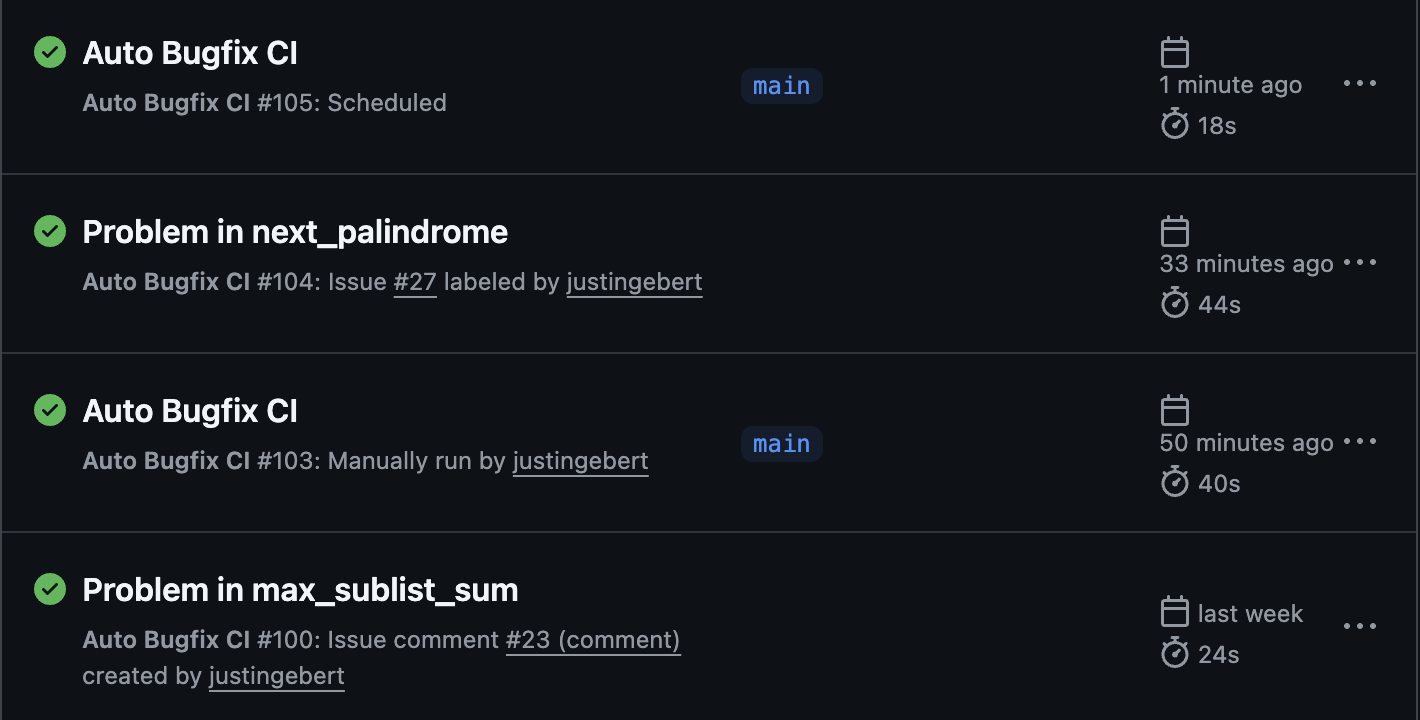
\includegraphics[width=1\textwidth]{images/verification/triggers.png}
    \caption{Workflow triggers for APR system}
    \label{fig:triggers}
\end{figure}

\begin{lstlisting}[style=log, caption={Filtered issues log excerpt}, label={lst:filtered-issues}, basicstyle=\ttfamily\small, breaklines=true, frame=single, columns=fullflexible]
Found 1 issues to process
[{"number": 27, "title": "Problem in next_palindrome", "body": "There is a bug in **`next_palindrome`**.", "labels": ["bug_v01", "quixbugs"]}]
\end{lstlisting}

\begin{lstlisting}[style=log, caption={Code checkout log excerpt}, label={fig:code-checkout}, basicstyle=\ttfamily\small, breaklines=true, frame=single, columns=fullflexible]
Run actions/checkout@v4
Syncing repository: justingebert/bugfix-ci
Getting Git version info
Temporarily overriding HOME='/home/runner/work/_temp/6ca8e386-1931-4130-8b38-cd4993a6fa1f' before making global git config changes
Adding repository directory to the temporary git global config as a safe directory
/usr/bin/git config --global --add safe.directory /home/runner/work/bugfix-ci/bugfix-ci
Deleting the contents of '/home/runner/work/bugfix-ci/bugfix-ci'
Initializing the repository
Disabling automatic garbage collection
Setting up auth
Fetching the repository
Determining the checkout info
/usr/bin/git sparse-checkout disable
/usr/bin/git config --local --unset-all extensions.worktreeConfig
Checking out the ref
/usr/bin/git log -1 --format=%H
465a84dc8a989cd1ba7603324687f7d57cdc0998
\end{lstlisting}

\begin{lstlisting}[style=log, caption={Bug localization log excerpt}, label={lst:loc}]
root - INFO - [localize] LLM response: ["next_palindrome.py"]
\end{lstlisting}

\begin{lstlisting}[style=json, caption={Fix generation log excerpt}, label={fig:fix}]
    "fix_attempt_1": {
        "results": {
          "status": "success",
          "message": "Successfully fixed files",
          "details": {
            "fixed_files": [
              "/workspace/quixbugs/python_programs/next_palindrome.py"
            ],
            "tokens": {
              "input_tokens": 431,
              "output_tokens": 288,
              "total_tokens": 719,
              "cost": 0.0006332
            },
            "raw_response": "=== File: /workspace/quixbugs/python_programs/next_palindrome.py ===\ndef next_palindrome(digit_list):\n    high_mid = len(digit_list) // 2\n    low_mid = (len(digit_list) - 1) // 2\n    while high_mid < len(digit_list) and low_mid >= 0:\n        if digit_list[high_mid] == 9:\n            digit_list[high_mid] = 0\n            digit_list[low_mid] = 0\n            high_mid += 1\n            low_mid -= 1\n        else:\n            digit_list[high_mid] += 1\n            if low_mid != high_mid:\n                digit_list[low_mid] = digit_list[high_mid]\n            return digit_list\n    return [1] + (len(digit_list) - 1) * [0] + [1]\n\n\"\"\"\nFinds the next palindromic integer when given the current integer\nIntegers are stored as arrays of base 10 digits from most significant to least significant\n\nInput:\n    digit_list: An array representing the current palindrome\n\nOutput:\n    An array which represents the next palindrome\n\nPreconditions:\n    The initial input array represents a palindrome\n\nExample\n    >>> next_palindrome([1,4,9,4,1])\n    [1,5,0,5,1]\n\"\"\""
          }
        },
        "duration": 7.0682
      },
\end{lstlisting}

\begin{lstlisting}[style=log, caption={Change validation log excerpt}, label={fig:validation}]
    root - INFO - == Running stage: build ==
    root - INFO - [build] starting build process 
    root - INFO - [build] Formatting /workspace/quixbugs/python_programs/next_palindrome.py with black...
    root - INFO - [build] /workspace/quixbugs/python_programs/next_palindrome.py formatted successfully by black.
    root - INFO - [build] Linting /workspace/quixbugs/python_programs/next_palindrome.py with flake8...
    root - WARNING - [build] flake8 found issues in /workspace/quixbugs/python_programs/next_palindrome.py:
    /workspace/quixbugs/python_programs/next_palindrome.py:20:80: E501 line too long (90 > 79 characters)
    
    root - ERROR - [build] Build failed. 1 files with issues.
    root - INFO - == Stage build completed in 0.5411 seconds ==
    root - INFO - == Running stage: test ==
    root - INFO - [test] running tests for fixed files
    root - INFO - [test] Testing next_palindrome...
    root - INFO - [test] Looking for specific test: /workspace/quixbugs/python_testcases/test_next_palindrome.py
    root - INFO - [test] Executing test command: cd /workspace/quixbugs && python -m pytest python_testcases/test_next_palindrome.py -v
    root - INFO - [test] Specific test passed for next_palindrome.
\end{lstlisting}

\begin{lstlisting}[style=log, caption={Iterative patch generation log excerpt}, label={fig:retry}]
    root - INFO - [test] Specific test failed for wrap.
    root - ERROR - [test] Tests failed. 1 files with test failures.
    root - INFO - == Stage test completed in 0.5417 seconds ==
    root - INFO - === Repair failed on attempt 1/3, trying again ===
    root - INFO - Resetting to main branch
    root - INFO - Reset /workspace/python_programs/wrap.py to main branch
    root - INFO - === Attempt 2/3 for issue #47 ===
    root - INFO - == Running stage: fix ==
    root - INFO - Loaded file: /workspace/python_programs/wrap.py
\end{lstlisting}

\begin{lstlisting}[style=log, caption={Branch and commit created for bugfix}, label={lst:branch-commit}]
    root - INFO - === Repair successful on attempt 1/1 ===
    root - INFO - Added file /workspace/quixbugs/python_programs/next_palindrome.py to staging area
    root - INFO - 1 files with changes committed to branch bugfix_v01_27
    root - INFO - Push successful
\end{lstlisting}


\begin{figure}[H]
    \centering
    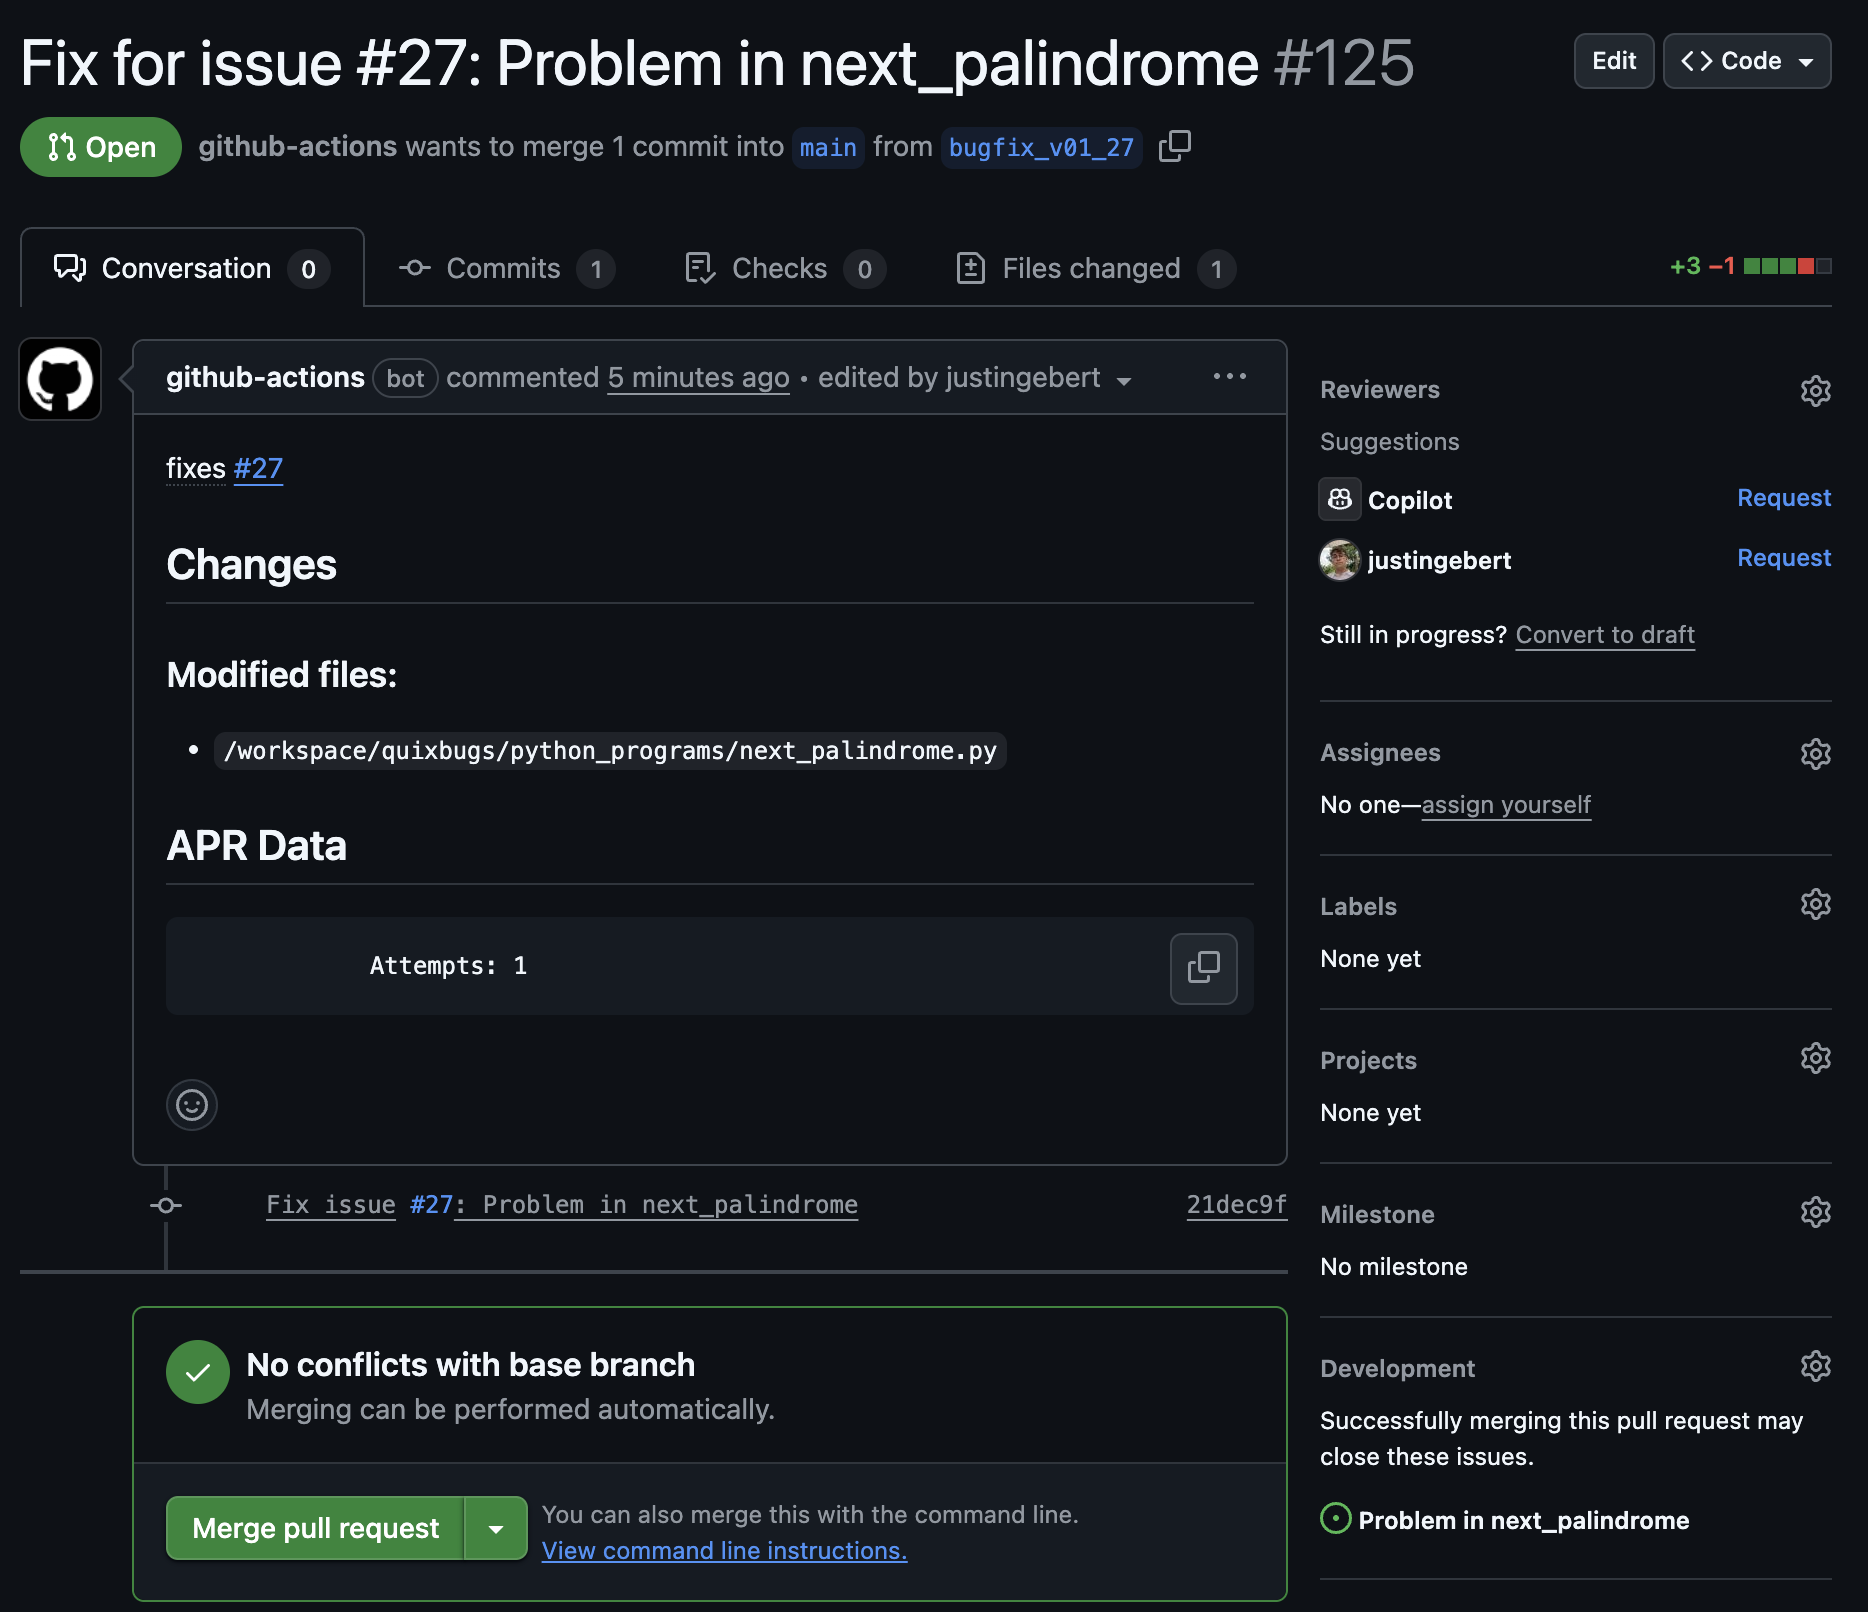
\includegraphics[width=1\textwidth]{images/verification/pr.png}
    \caption{Pull request report for bugfix}
    \label{fig:pr-report}
\end{figure}

\begin{figure}[H]
    \centering
    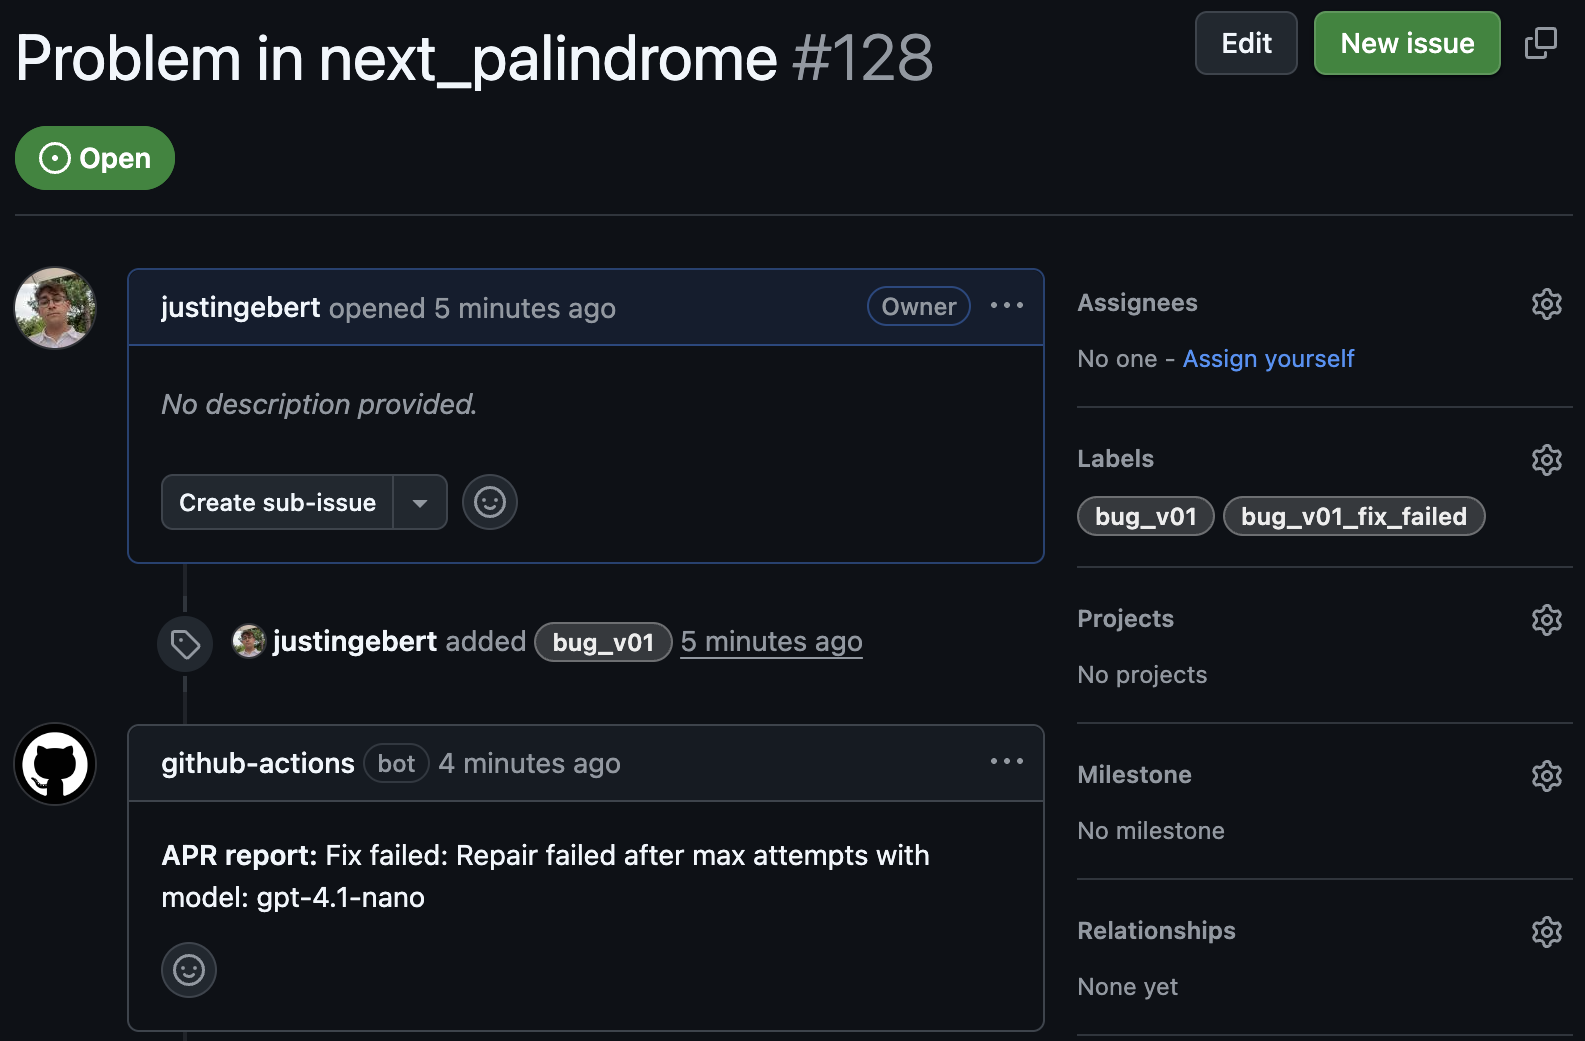
\includegraphics[width=1\textwidth]{images/verification/comment.png}
    \caption{Issue comment reporting repair result}
    \label{fig:comment}
\end{figure}

\begin{figure}[H]
    \centering
    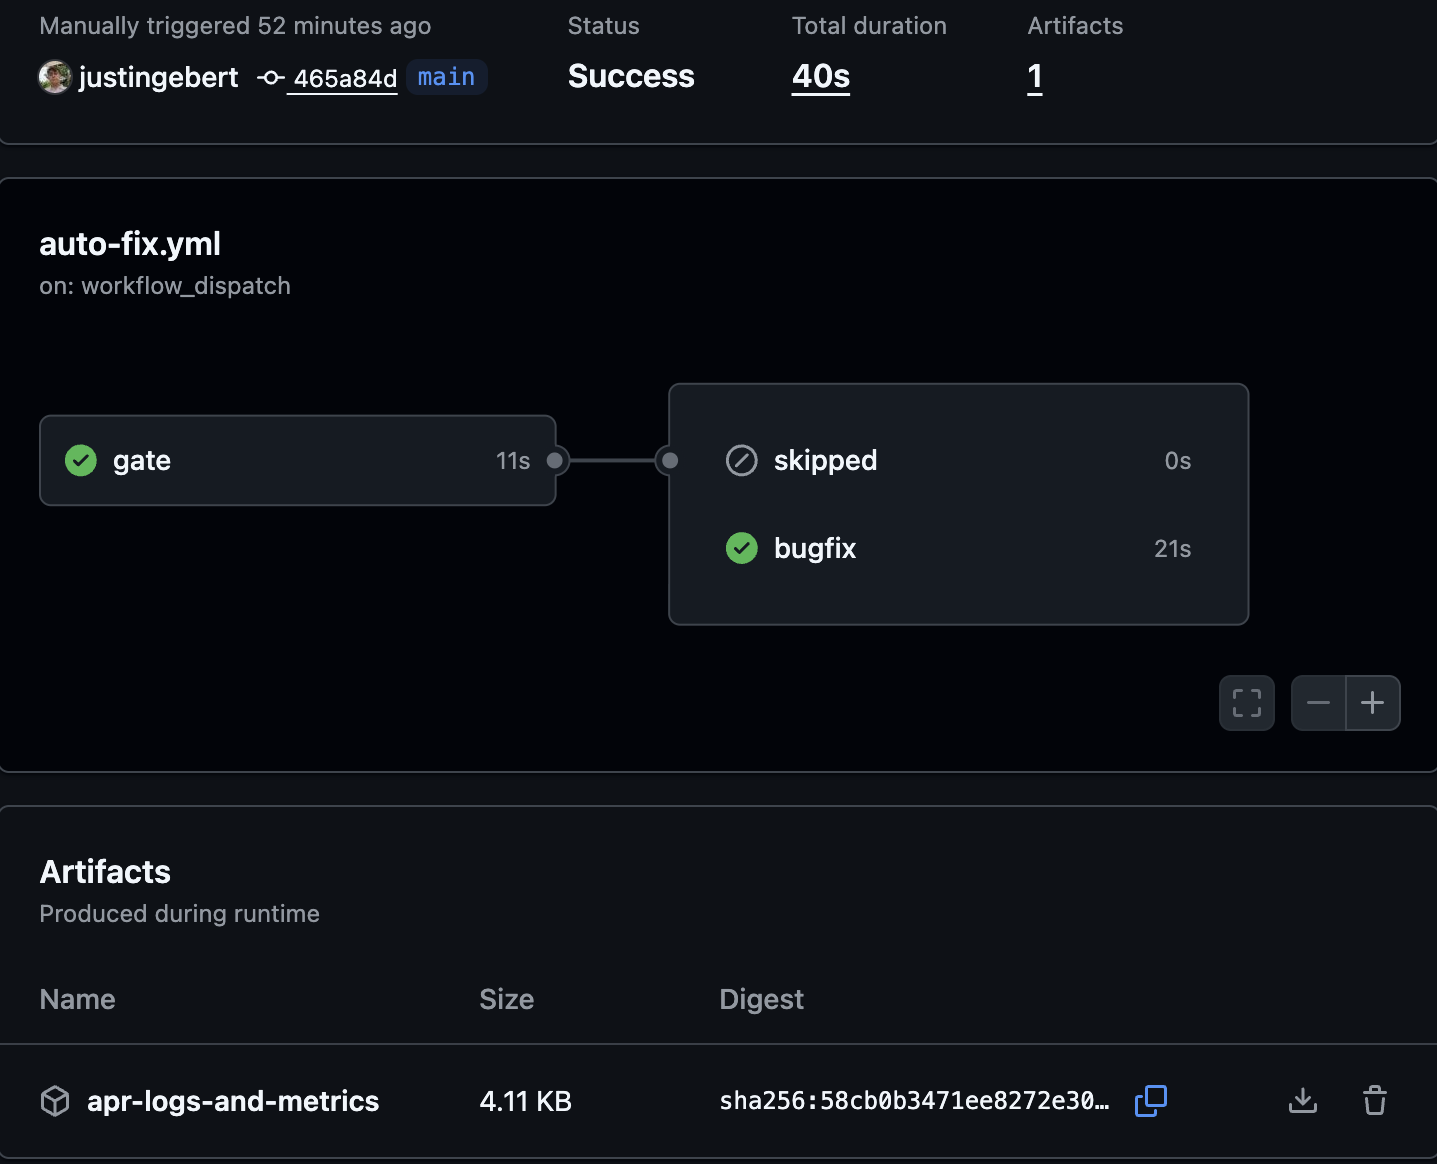
\includegraphics[width=1\textwidth]{images/verification/artifacts.png}
    \caption{Downloadable Artifacts from workflow run}
    \label{fig:logs-artifacts}
\end{figure}

\begin{lstlisting}[style=log, caption={Docker container runtime log excerpt}, label={lst:docker-log}]
    Downloaded newer image for ghcr.io/justingebert/bugfix-ci:latest
    Run docker run --rm \
    docker run --rm \
      -v "$GITHUB_WORKSPACE:/workspace" \
      -e GITHUB_TOKEN -e GITHUB_RUN_ID -e GITHUB_REPOSITORY -e LLM_API_KEY -e FILTERED_ISSUES \
      ghcr.io/justingebert/bugfix-ci:latest
    shell: /usr/bin/bash -e {0}
    env:
      GITHUB_TOKEN: ***
      GITHUB_REPOSITORY: justingebert/bugfix-ci
      GITHUB_RUN_ID: 16531173399
      LLM_API_KEY: ***
      FILTERED_ISSUES: [{"number": 27, "title": "Problem in next_palindrome", "body": "There is a bug in **`next_palindrome`**.\n\n* **File**: `/Users/justingebert/Projects/Uni/BA/bugfix-ci/datasets/quixbugs/python_programs/next_palindrome.py`", "labels": ["bug_v01", "quixbugs"]}]
\end{lstlisting}

\begin{lstlisting}[style=log, caption={Load custom configuration}, label={lst:load-config}]
    root - INFO - [info] loaded default config from apr_core/default-config.yml
    root - INFO - [info] loaded config from /workspace/bugfix.yml
\end{lstlisting}